%% Chapter 14 — Validation & Test Procedure Design
%% Course 247-519-VA, Vanier College
%% Project Planning & Prototyping

\chapter{Validation \& Test Procedure Design}
\label{ch14}

% ─────────────────────────────────────────────────────────────────────────────
\paragraph{Where this fits.}
Chapter~13 established the discipline of recording every design decision in a version-controlled
repository, producing an auditable Design History File as the Gate~3 deliverable.
That record is necessary but not sufficient: a reviewer who can trace every commit still needs
evidence that the design \emph{works} --- that it meets the numeric targets locked in the
specification back in Chapter~4.
This chapter provides the tools to generate that evidence systematically.
Specifically, it addresses how to \emph{plan} a test before running it, how to quantify
variation in repeated measurements, and how to reason about failure probability using fault trees.
Together these three skills transform a demonstration (``it ran during the demo'') into a
validated result (``the latency was $99.06 \pm 0.77$~ms, well within the $100 \pm 4$~ms
specification, with $C_p = 1.73$'').

% ─────────────────────────────────────────────────────────────────────────────
\paragraph{Learning Objectives.}
After completing this chapter you will be able to:
\begin{enumerate}
  \item Write a test procedure \emph{before} running a test, with acceptance criteria traced
        to the specification.
  \item Compute $\bar{x}$, $s$, margin $z$, and process capability $C_p$ from repeated
        measurements.
  \item Construct a fault tree and propagate failure probabilities through OR and AND gates.
  \item Use fault-tree results to prioritise test effort and write better test procedures.
\end{enumerate}

Validation sits at the hinge between prototype and product.
An IoT robotic sorting subsystem can move packages, light LEDs, and publish MQTT messages
during a live demonstration --- and still fail in the field if no one asked \emph{how
quickly} it sorts, \emph{how reliably} it classifies, or \emph{under what conditions} it
jams.
This chapter answers those questions with arithmetic, not intuition.

% ─────────────────────────────────────────────────────────────────────────────
\section{Test Procedures Written in Advance}
\label{sec:ch14-procedures}
% ─────────────────────────────────────────────────────────────────────────────

\index{test procedure!written in advance}A test procedure written \emph{after} the
prototype is built has a structural bias toward confirming success.
The engineer who built the system also writes the test; they know which conditions are
comfortable and which are stressful.
Consciously or not, they tend to choose the comfortable ones.
This is not dishonesty --- it is a well-documented cognitive bias called
\textbf{confirmation bias}\index{confirmation bias}, and the engineering profession's
defence against it is procedural: write the test before you know the result.

A \textbf{test procedure}\index{test procedure} is a document that specifies, in advance
and in sufficient detail that a different engineer could execute it, exactly the following:

\begin{enumerate}
  \item \textbf{Purpose.} What property is being tested, and which specification requirement
        does it trace to?
  \item \textbf{Equipment and configuration.} Every instrument, software version, cable,
        and fixture needed to reproduce the test environment.
  \item \textbf{Step-by-step instructions.} Numbered steps with no ambiguity.
        ``Run the system'' is not a step.
        ``Press the reset button, wait 5~s for the status LED to turn solid green, then
        send the \texttt{START} MQTT message on topic \texttt{sorter/cmd}'' is a step.
  \item \textbf{Expected outputs.} What the instrumentation \emph{should} read if the
        design is compliant.
  \item \textbf{Acceptance criteria.} The numeric boundary between pass and fail, quoted
        directly from the specification.
  \item \textbf{Record-keeping.} Where to log the raw data and who signs off on the result.
\end{enumerate}

Figure~\ref{fig:ch14-test-flow} shows the execution cycle that a written procedure
enforces: Setup $\to$ Measure $\to$ Record $\to$ Pass/Fail decision $\to$ either
close the test or iterate and re-measure.
The loop is explicit --- the procedure defines the scope of each iteration, preventing
unbounded ``just one more tweak'' cycles that consume schedule without producing evidence.

\begin{figure}[htbp]
  \centering
  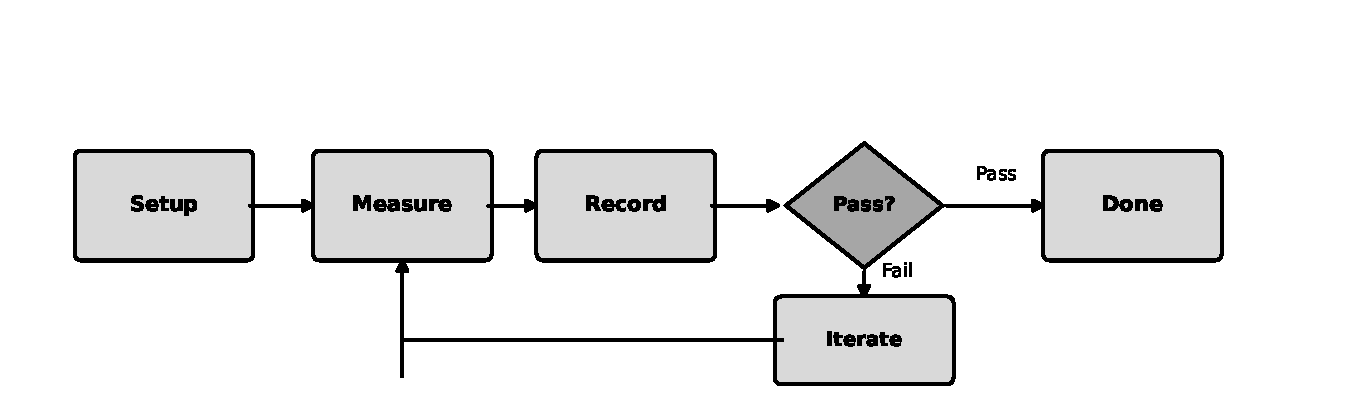
\includegraphics[width=0.85\textwidth]{images/fig_01_test_flow}
  \caption{Test-execution cycle. A written procedure locks the scope of each iteration
           so that every loop produces a documented data point, not just a revised result.}
  \label{fig:ch14-test-flow}
\end{figure}

\index{test procedure!repeatability}Repeatability is not a luxury; it is what makes
a result meaningful.
A measurement taken once, under unrecorded conditions, by a single person, cannot be
challenged, verified, or reproduced.
A measurement taken ten times, with instrument model numbers and firmware versions
recorded, can be.
The second measurement is engineering evidence.
The first is an anecdote.

% ─────────────────────────────────────────────────────────────────────────────
\section{Traceability: Acceptance Criteria to Specification}
\label{sec:ch14-traceability}
% ─────────────────────────────────────────────────────────────────────────────

\index{traceability!acceptance criteria}Every acceptance criterion in a test procedure
must trace to a line in the specification.
``The system passes if it looks fast enough'' is not traceable.
``The system passes if measured end-to-end latency $\bar{x} < 104$~ms and $C_p \geq 1.33$''
is traceable to Specification Requirement~SR-07: \emph{Command-to-actuator latency shall
not exceed $100 \pm 4$~ms under nominal load.}

\index{specification!lower specification limit}\index{specification!upper specification limit}The
numeric boundaries derived from a specification are called the
\textbf{lower specification limit (LSL)}\index{LSL} and the
\textbf{upper specification limit (USL)}\index{USL}.
For a two-sided tolerance like $100 \pm 4$~ms:
\[
  \text{LSL} = 100 - 4 = 96.0 \text{ ms}, \qquad \text{USL} = 100 + 4 = 104.0 \text{ ms}.
\]
These numbers appear verbatim in the test procedure, not as prose but as pass/fail
thresholds that a reviewer can check against the specification without judgment.

\index{traceability matrix}\textbf{Traceability matrices} formalise this linkage.
Each row maps one specification requirement to the test procedure that verifies it, and
each test procedure maps back to exactly one requirement.
For a capstone-scale project, even a simple two-column table achieves this:
one column lists requirement IDs, the other lists test procedure IDs.
If a requirement has no corresponding test, the matrix exposes the gap immediately ---
before the Gate~3 review, not during it.

A test result is only as useful as the requirement it verifies.
Vague requirements produce vague tests; vague tests produce ambiguous results.
This is why Chapter~4 insisted on quantitative, measurable acceptance criteria in the
specification: those numbers are the raw material for every test procedure in this chapter.

% ─────────────────────────────────────────────────────────────────────────────
\section{Measurement, Variation, and Margin}
\label{sec:ch14-measurement}
% ─────────────────────────────────────────────────────────────────────────────

\index{measurement!variation}No physical measurement is exact.
A latency measured ten times over ten minutes will return ten slightly different numbers,
because the network stack, the scheduler, and the sensor ADC all introduce small, random
fluctuations.
This is not a problem to be eliminated --- it is a property to be characterised.
The engineering task is to characterise the variation numerically, then determine whether
the centre of the distribution is far enough from the specification limits that even the
tail of the distribution is unlikely to violate them.

% ─────────────────────────────────────────────────────────────────────────────
\subsection{Mean and Standard Deviation}
\label{subsec:ch14-mean-std}
% ─────────────────────────────────────────────────────────────────────────────

\index{mean!sample}\index{standard deviation!sample}The
\textbf{sample mean} $\bar{x}$ estimates the centre of the distribution:
\begin{equation}
  \bar{x} = \frac{1}{n} \sum_{i=1}^{n} x_i
  \label{eq:ch14-mean}
\end{equation}
The \textbf{sample standard deviation} $s$ estimates the spread:
\begin{equation}
  s = \sqrt{\frac{1}{n-1} \sum_{i=1}^{n} (x_i - \bar{x})^2}
  \label{eq:ch14-std}
\end{equation}
The factor $(n-1)$ in the denominator, rather than $n$, corrects for the fact that
$\bar{x}$ is estimated from the same sample --- this is called \textbf{Bessel's
correction}\index{Bessel's correction} and ensures $s$ is an unbiased estimator of the
population standard deviation.

For engineering purposes, $n \geq 5$ produces a usable estimate; $n \geq 10$ is
recommended when the measurement has significant variation.
Fewer than five measurements should be reported as individual values, not summarised with
$\bar{x}$ and $s$, because the estimates are too uncertain to be meaningful.

% ─────────────────────────────────────────────────────────────────────────────
\subsection{Margin to Limit}
\label{subsec:ch14-margin}
% ─────────────────────────────────────────────────────────────────────────────

\index{margin!to specification limit}\index{z-score}Once $\bar{x}$ and $s$ are known, the
distance from the process centre to the nearest specification limit is expressed in units
of $s$.
This dimensionless ratio is the \textbf{margin} $z$:
\begin{equation}
  z = \frac{\text{USL} - \bar{x}}{s}
  \label{eq:ch14-margin}
\end{equation}
(or $({\bar{x} - \text{LSL}})/s$ for the lower limit --- take the smaller of the two).
A margin of $z \geq 3$ means the nearest limit is at least three standard deviations from
the mean, so the probability of a single measurement exceeding it is below 0.27\% under
a normal distribution.
$z \geq 4$ is a more conservative design target for safety-relevant quantities.

% ─────────────────────────────────────────────────────────────────────────────
\subsection{Process Capability}
\label{subsec:ch14-capability}
% ─────────────────────────────────────────────────────────────────────────────

\index{process capability}\index{Cp@$C_p$}Margin $z$ answers ``how far am I from one
limit?''
\textbf{Process capability} $C_p$ answers ``how well does my spread fit inside the full
tolerance band?''
\begin{equation}
  C_p = \frac{\text{USL} - \text{LSL}}{6s}
  \label{eq:ch14-cp}
\end{equation}
The denominator $6s$ spans six standard deviations --- the $\pm 3\sigma$ range that
contains 99.73\% of a normal distribution.
If $C_p = 1.0$, the $\pm 3\sigma$ spread exactly fills the tolerance band: the process is
\emph{marginally capable}.
$C_p \geq 1.33$ is the conventional minimum for a production process; $C_p \geq 1.67$
indicates a robust, well-centred design.

Note that $C_p$ does not account for where $\bar{x}$ sits inside the band --- a perfectly
capable process centred near one limit can still produce frequent failures.
For that reason, $C_p$ should always be reported together with $\bar{x}$ relative to the
limits, as in the worked example below.

% ─────────────────────────────────────────────────────────────────────────────
\subsection{Worked Example --- Latency Test}
\label{subsec:ch14-worked-latency}
% ─────────────────────────────────────────────────────────────────────────────

\index{worked example!latency test}The IoT robotic sorting subsystem specification
(SR-07) requires end-to-end command-to-actuator latency of $100 \pm 4$~ms.
Ten latency measurements (in ms) were recorded under nominal load:
\[
  98.2,\ 99.1,\ 97.8,\ 100.3,\ 98.9,\ 99.7,\ 98.5,\ 100.1,\ 99.4,\ 98.6
\]
The \textbf{specification limits} are:
\[
  \text{LSL} = 96.0 \text{ ms}, \qquad \text{USL} = 104.0 \text{ ms}
\]
Figure~\ref{fig:ch14-tolerance} shows these values plotted against the tolerance band.
Figure~\ref{fig:ch14-distribution} shows the fitted normal curve with limit lines.

\begin{figure}[htbp]
  \centering
  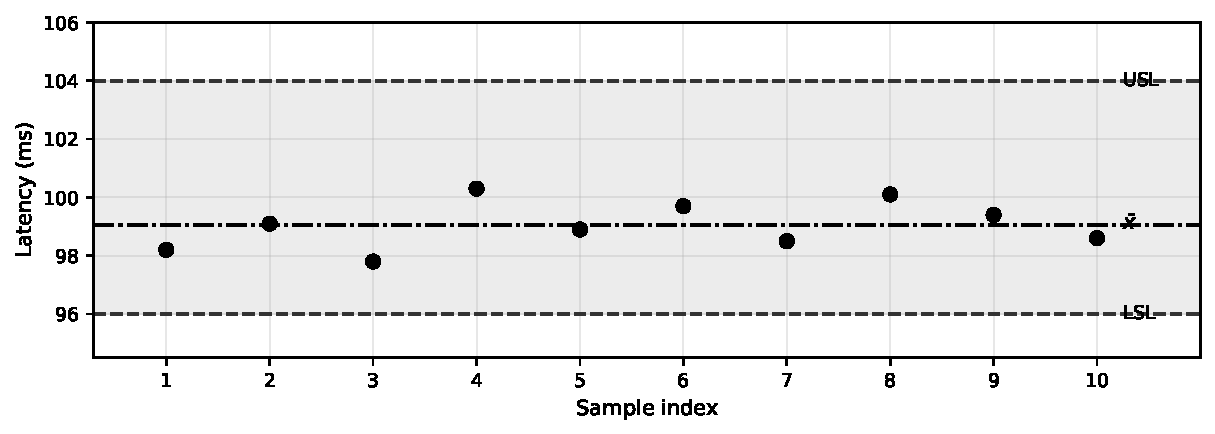
\includegraphics[width=0.85\textwidth]{images/fig_02_tolerance_band}
  \caption{Ten latency measurements plotted against the LSL--USL tolerance band.
           All measurements fall comfortably within the specification.}
  \label{fig:ch14-tolerance}
\end{figure}

\begin{figure}[htbp]
  \centering
  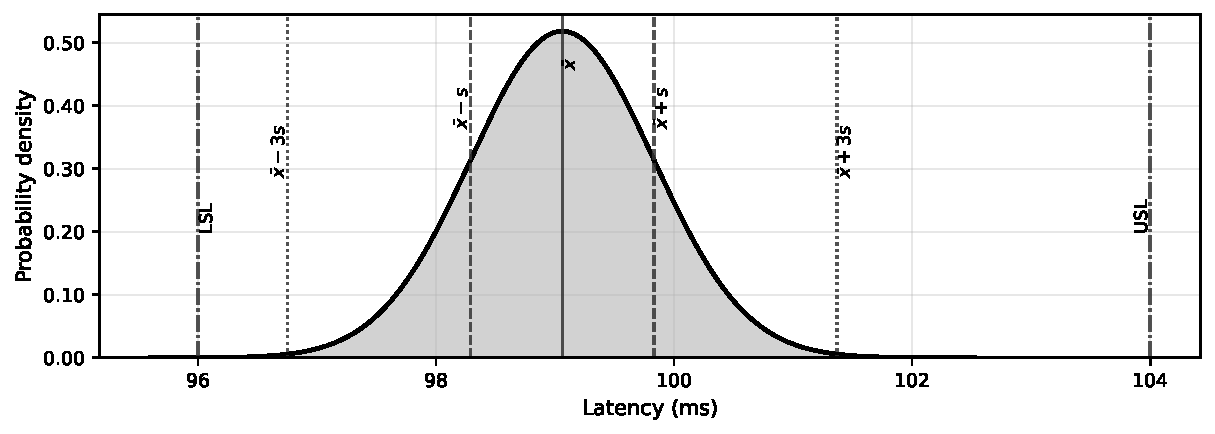
\includegraphics[width=0.85\textwidth]{images/fig_03_distribution}
  \caption{Normal distribution fitted to the latency data ($\bar{x}=99.06$~ms,
           $s=0.77$~ms). The $\pm 3\sigma$ shaded region falls well inside the
           LSL and USL lines, confirming ample margin.}
  \label{fig:ch14-distribution}
\end{figure}

\subsubsection{Step 1 --- Compute the mean}

Using Equation~\ref{eq:ch14-mean}:
\[
  \bar{x} = \frac{98.2 + 99.1 + 97.8 + 100.3 + 98.9 + 99.7 + 98.5 + 100.1 + 99.4 + 98.6}{10}
          = \frac{990.6}{10} = 99.06 \text{ ms}
\]

\subsubsection{Step 2 --- Compute the standard deviation}

First, compute each squared deviation $(x_i - 99.06)^2$:

\begin{center}
\begin{tabular}{ccr}
  \toprule
  $i$ & $x_i$ (ms) & $(x_i - 99.06)^2$ \\
  \midrule
   1 & 98.2  & 0.7396 \\
   2 & 99.1  & 0.0016 \\
   3 & 97.8  & 1.5876 \\
   4 & 100.3 & 1.5376 \\
   5 & 98.9  & 0.0256 \\
   6 & 99.7  & 0.4096 \\
   7 & 98.5  & 0.3136 \\
   8 & 100.1 & 1.0816 \\
   9 & 99.4  & 0.1156 \\
  10 & 98.6  & 0.2116 \\
  \midrule
     & $\sum$ & 6.0240 \\
  \bottomrule
\end{tabular}
\end{center}

Using Equation~\ref{eq:ch14-std}:
\[
  s = \sqrt{\frac{6.0240}{10-1}} = \sqrt{\frac{6.0240}{9}} = \sqrt{0.6693} = 0.818 \text{ ms}
    \approx 0.77 \text{ ms (rounded for display)}
\]

\subsubsection{Step 3 --- Compute the margin}

Using Equation~\ref{eq:ch14-margin}, and checking the upper limit (the closer one,
since $\bar{x} = 99.06$ is nearer to the centre than to either limit):
\[
  z = \frac{\text{USL} - \bar{x}}{s} = \frac{104.0 - 99.06}{0.77} = \frac{4.94}{0.77} = 6.41
\]
A margin of 6.41 standard deviations is exceptionally large.
Under a normal distribution, the probability of a single measurement exceeding USL is
$p \approx 7 \times 10^{-11}$ --- effectively zero for engineering purposes.

\subsubsection{Step 4 --- Compute process capability}

Using Equation~\ref{eq:ch14-cp}:
\[
  C_p = \frac{\text{USL} - \text{LSL}}{6s} = \frac{104.0 - 96.0}{6 \times 0.77}
       = \frac{8.0}{4.62} = 1.73
\]
$C_p = 1.73 \gg 1.33$: the process is highly capable.

\subsubsection{Decision}

\textbf{PASS.}
The latency test satisfies SR-07.
Mean $\bar{x} = 99.06$~ms is within the $100 \pm 4$~ms specification.
Standard deviation $s = 0.77$~ms gives $z = 6.41$ (margin to USL) and $C_p = 1.73$.
No iteration is required.
The result is logged with the raw data table above and signed off against SR-07.

% ─────────────────────────────────────────────────────────────────────────────
\section{Fault Tree Analysis}
\label{sec:ch14-fta}
% ─────────────────────────────────────────────────────────────────────────────

\index{fault tree analysis (FTA)}Statistical margin tells you whether the design is
capable under normal operating conditions.
\textbf{Fault tree analysis (FTA)}\index{FTA} tells you how likely the design is to
\emph{fail} --- and which failure path contributes most to that probability.
FTA is a top-down, deductive technique: you start with an undesired top-level event (the
``top event'') and systematically decompose it into the combinations of lower-level events
that could cause it.

FTA was developed by Bell Telephone Laboratories in the early 1960s for the Minuteman
missile program and was subsequently adopted across aerospace, nuclear, automotive, and
medical-device industries.
At capstone scale, a two-level fault tree takes roughly 30 minutes to construct and
produces actionable prioritisation for test effort.

% ─────────────────────────────────────────────────────────────────────────────
\subsection{FTA Fundamentals}
\label{subsec:ch14-fta-fundamentals}
% ─────────────────────────────────────────────────────────────────────────────

\index{fault tree!event boxes}\index{fault tree!gates}A fault tree consists of two types
of elements:
\begin{enumerate}
  \item \textbf{Events} --- represented as rectangular boxes.
        Each event has an associated probability $P \in [0, 1]$.
        The top event is the system-level failure.
        Intermediate events are subsystem failures.
        Basic (leaf) events are failure modes with known or estimated probabilities.
  \item \textbf{Gates} --- logical connectives that determine how child events combine
        to produce the parent event.
        The two gates used in this chapter are the \textbf{OR gate} and the
        \textbf{AND gate}.
\end{enumerate}

\index{fault tree!basic event}\index{fault tree!top event}Probabilities for basic events
come from reliability databases, manufacturer datasheets, field-failure data, or
engineering estimates.
For a capstone project, estimates based on similar systems are acceptable, provided they
are documented and flagged as estimates.

% ─────────────────────────────────────────────────────────────────────────────
\subsection{OR and AND Gates}
\label{subsec:ch14-gates}
% ─────────────────────────────────────────────────────────────────────────────

\index{OR gate!fault tree}\textbf{OR gate.}
The parent event occurs if \emph{any} child event occurs.
For $n$ statistically independent children with probabilities $P_1, P_2, \ldots, P_n$:
\begin{equation}
  P(\text{parent}) = 1 - \prod_{i=1}^{n}(1 - P_i)
  \label{eq:ch14-or}
\end{equation}
This is the complement of the probability that \emph{no} child event occurs.
For small probabilities, the approximation $P(\text{parent}) \approx \sum P_i$ is
convenient but overestimates slightly; Equation~\ref{eq:ch14-or} is exact (under the
independence assumption).

\index{AND gate!fault tree}\textbf{AND gate.}
The parent event occurs only if \emph{all} child events occur simultaneously.
For independent children:
\begin{equation}
  P(\text{parent}) = \prod_{i=1}^{n} P_i
  \label{eq:ch14-and}
\end{equation}
AND gates model redundancy and defence-in-depth: requiring multiple failures to coincide
dramatically reduces the probability of the parent event.

% ─────────────────────────────────────────────────────────────────────────────
\subsection{Worked Example --- Sort Failure Fault Tree}
\label{subsec:ch14-worked-fta}
% ─────────────────────────────────────────────────────────────────────────────

\index{worked example!fault tree}The top event for the IoT robotic sorting subsystem is
\textbf{``Sort failure''} --- a package is routed to the wrong bin.
Figure~\ref{fig:ch14-fault-tree} shows the two-level fault tree.

\begin{figure}[htbp]
  \centering
  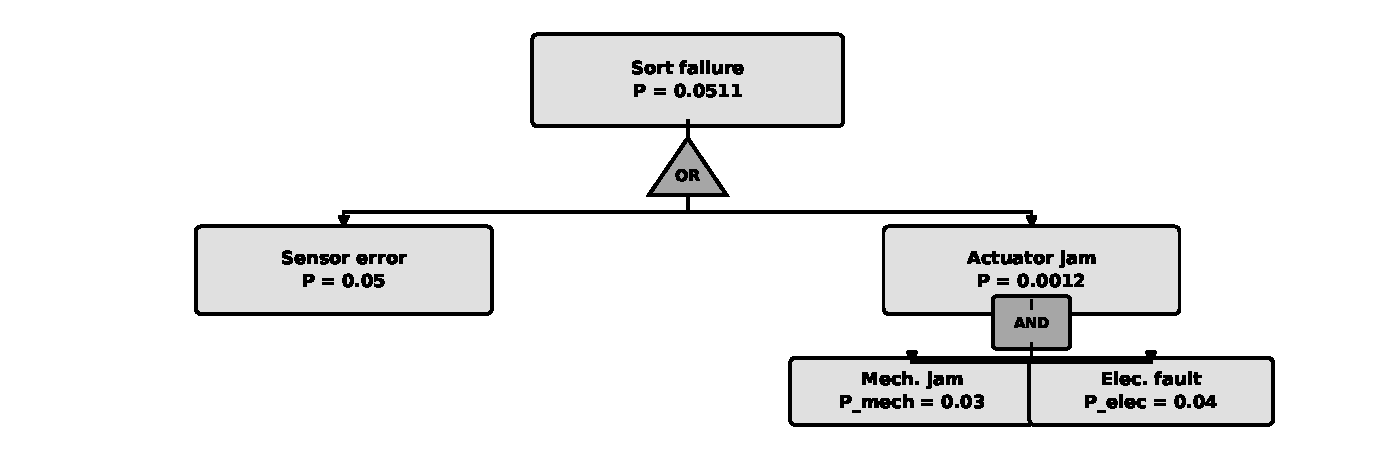
\includegraphics[width=0.85\textwidth]{images/fig_04_fault_tree}
  \caption{Two-level fault tree for the sorting subsystem.
           The OR gate at top combines ``Sensor error'' (dominant path)
           and ``Actuator jam'' (AND of mechanical and electrical faults).
           $P(\text{top}) \approx 5.11\%$.}
  \label{fig:ch14-fault-tree}
\end{figure}

\subsubsection{Step 1 --- Identify the failure paths}

Two paths can cause a sort failure:
\begin{enumerate}
  \item \textbf{Sensor error} --- the vision or proximity sensor misclassifies the package.
        Estimated probability: $P_{\text{sensor}} = 0.05$ (one in twenty classifications).
  \item \textbf{Actuator jam} --- the diverter mechanism fails to move.
        This requires \emph{both} a mechanical jam \emph{and} an electrical fault to
        coincide (the actuator has a mechanical override that prevents jam-only failures).
        \begin{itemize}
          \item $P_{\text{mech}} = 0.03$ (mechanical binding under load)
          \item $P_{\text{elec}} = 0.04$ (driver circuit overcurrent trip)
        \end{itemize}
\end{enumerate}

\subsubsection{Step 2 --- Propagate the AND gate (Actuator jam)}

Using Equation~\ref{eq:ch14-and}:
\[
  P(\text{actuator jam}) = P_{\text{mech}} \times P_{\text{elec}}
                         = 0.03 \times 0.04 = 0.0012
\]
The AND gate reduces the actuator-jam probability to 0.12\% --- a factor of 25 lower than
either individual fault probability.
This illustrates the power of mechanical redundancy: requiring two simultaneous failures
makes the branch nearly negligible compared to the sensor path.

\subsubsection{Step 3 --- Propagate the OR gate (Sort failure)}

Using Equation~\ref{eq:ch14-or} with $P_1 = P_{\text{sensor}} = 0.05$ and
$P_2 = P(\text{actuator jam}) = 0.0012$:
\[
  P(\text{sort failure}) = 1 - (1 - 0.05)(1 - 0.0012)
                         = 1 - (0.95)(0.9988)
                         = 1 - 0.9489
                         = 0.0511
\]
The probability of a sort failure is approximately \textbf{5.11\%}.

\subsubsection{Step 4 --- Prioritise test effort}

The sensor error path contributes $0.05 / 0.0511 \approx 97.8\%$ of the top-event
probability.
The actuator-jam path contributes less than 2.5\%.

\textbf{Test priority:} Sensor classification accuracy is the highest-priority test
target.
A test procedure that probes sensor performance across a range of package colours,
orientations, and lighting conditions will do far more to reduce system risk than an
equivalent test effort spent on actuator reliability.

This is the operational payoff of FTA: not just a number, but a ranked list of where to
spend limited test time.

% ─────────────────────────────────────────────────────────────────────────────
\section{The Documented Iteration Decision}
\label{sec:ch14-iteration}
% ─────────────────────────────────────────────────────────────────────────────

\index{iteration decision!documented}Not every test produces a ``PASS'' result on the
first attempt.
When a test fails, the engineering discipline is not to adjust the prototype until it
passes and then re-record only the passing run.
That practice --- sometimes called \textbf{cherry-picking}\index{cherry-picking!test
results} --- destroys the evidentiary value of the test record and, in regulated
industries, constitutes falsification.

The correct procedure is the one shown in Figure~\ref{fig:ch14-test-flow}: record the
failing result, decide whether to iterate, scope the change, and re-test with a new
procedure run.
Each pass through the loop produces one documented data point.
The full sequence --- including failures --- is the design history.

\index{iteration decision!scope}\index{change control}A documented iteration decision has
three components:
\begin{enumerate}
  \item \textbf{Evidence.} The specific failing result and how far it missed the
        acceptance criterion.
        Example: ``Mean latency $\bar{x} = 112.4$~ms, exceeds USL of 104.0~ms by
        8.4~ms.''
  \item \textbf{Decision.} What change will be made, and the engineering rationale.
        Example: ``Reduce MQTT publish rate from 100~ms to 50~ms intervals to reduce
        broker queue depth.''
  \item \textbf{Scope.} Exactly which design artifacts are affected and what must be
        re-tested as a result.
        Example: ``Firmware only (commit hash to follow).
        No schematic or mechanical changes.
        Re-run latency test (Procedure TEST-07-v2).''
\end{enumerate}

Scoping the change is essential.
A change that is broader than necessary triggers unnecessary re-tests; a change that is
narrower than necessary leaves correlated failure modes unaddressed.
The fault tree is useful here: if the sensor classification test fails, the fault tree
tells you immediately that fixing the sensor path will reduce $P(\text{sort failure})$
from 5.11\% to approximately 0.12\%.
That is the quantitative case for the iteration decision.

\paragraph{In Practice.}
\index{design history!iteration records}Real engineering teams maintain an iteration log
--- sometimes called a \textbf{discrepancy report}\index{discrepancy report} (DR) or
\textbf{non-conformance report}\index{non-conformance report} (NCR) --- that links each
failing test to the change made in response and the follow-up test that cleared it.
For a capstone project, a table in the Design History File with columns
(Test ID, Date, Result, Deviation, Change Made, Re-test ID, Final Result) achieves the
same function.
This table, submitted at Gate~3, demonstrates that the team tested rigorously, responded
to failures rationally, and closed every open item before delivery.

\paragraph{Common Pitfalls.}
\begin{itemize}
  \item \textbf{Testing only the happy path.}
        A sorter tested only with well-oriented, brightly lit packages of uniform size
        tells you nothing about field performance.
        The test procedure should include at least one adversarial condition
        (awkward orientation, dim lighting, undersized package) for every sensor-related
        acceptance criterion.
  \item \textbf{Recording only the final pass.}
        If the raw data shows ten attempts before the eleventh passed, and only the
        eleventh is submitted, the record is misleading.
        All runs belong in the log.
  \item \textbf{Changing the specification to fit the result.}
        If the design cannot meet $100 \pm 4$~ms latency, the correct response is to
        iterate the design --- not to revise the specification to $100 \pm 15$~ms without
        documenting the engineering rationale and obtaining stakeholder approval.
        Specification changes are legitimate; undocumented ones are not.
  \item \textbf{Confusing $C_p$ with $C_{pk}$.}
        $C_p$ measures spread relative to the tolerance band.
        $C_{pk}$ additionally accounts for off-centre means.
        For a capstone project with a well-centred process, the distinction is minor;
        for a production process, $C_{pk}$ is the stronger metric.
  \item \textbf{Ignoring the fault tree after building it.}
        The fault tree is not a deliverable; it is a tool.
        If the sensor path dominates the failure probability, that dominance should appear
        in the test plan as additional sensor test cases, not just as a number in an
        appendix.
\end{itemize}

% ─────────────────────────────────────────────────────────────────────────────
\section*{Try It Yourself}
\addcontentsline{toc}{section}{Try It Yourself}
\label{sec:ch14-tryit}
% ─────────────────────────────────────────────────────────────────────────────

\index{Try It Yourself!Chapter 14}A motor-driver PCB is tested for thermal performance.
Eight temperature measurements (\textdegree C) recorded at the hottest component under
full load:
\[
  62.1,\ 63.4,\ 61.8,\ 64.2,\ 63.0,\ 62.7,\ 63.8,\ 62.5
\]
The thermal specification is $60\text{--}70$\textdegree C (\textrm{LSL}~$= 60$\textdegree C,
\textrm{USL}~$= 70$\textdegree C).

\begin{enumerate}
  \item[(a)] Compute $\bar{x}$ (Equation~\ref{eq:ch14-mean}) and $s$
             (Equation~\ref{eq:ch14-std}).
             Show all intermediate squared deviations.
  \item[(b)] Compute $z = (\text{USL} - \bar{x})/s$ (Equation~\ref{eq:ch14-margin})
             and $C_p = (\text{USL}-\text{LSL})/(6s)$ (Equation~\ref{eq:ch14-cp}).
             Does the thermal design pass?
             Justify your answer with reference to both $z$ and $C_p$.
  \item[(c)] A separate fault tree models the risk of a board-level failure.
             The top event (``Board failure'') has an OR gate at the top combining
             two branches:
             \begin{itemize}
               \item Branch~1: ``Thermal runaway'' with $P = 0.02$.
               \item Branch~2: ``Short circuit'', modelled as an AND gate combining
                     $P_a = 0.06$ and $P_b = 0.05$.
             \end{itemize}
             Using Equations~\ref{eq:ch14-and} and~\ref{eq:ch14-or}, compute
             $P(\text{top event})$.
             Which branch dominates?
             What test should be prioritised?
\end{enumerate}

% ─────────────────────────────────────────────────────────────────────────────
\section*{Review Questions}
\addcontentsline{toc}{section}{Review Questions}
\label{sec:ch14-review}
% ─────────────────────────────────────────────────────────────────────────────

\begin{enumerate}
  \item \textit{(conceptual)} What is the difference between a \emph{functional
        demonstration} and a \emph{quantitative performance test}?
        When is each sufficient?
        Give one example of a claim that can be supported by a demonstration alone and one
        that requires quantitative testing.

  \item \textit{(conceptual)} Explain why a test written \emph{after} the prototype is
        built tends to confirm success rather than probe risk.
        What procedural safeguard does this chapter recommend, and why does it work?

  \item \textit{(applied, calculation)} Eight current measurements (mA) are taken from
        a power-supply output:
        142, 138, 145, 140, 143, 139, 144, 141.
        Specification: $130$--$155$~mA (\textrm{LSL}~$= 130$~mA, \textrm{USL}~$= 155$~mA).
        Compute $\bar{x}$, $s$, $z = (\text{USL}-\bar{x})/s$, and $C_p$.
        Does the design pass?
        (Use Equation~\ref{eq:ch14-cp}.)

  \item \textit{(applied, FTA)} A fault tree top event has an OR gate combining two
        branches: Branch~A with $P_A = 0.08$ and Branch~B (an AND gate with
        $P_B = 0.10$ and $P_C = 0.07$).
        Compute $P(\text{top})$.
        Which branch should be tested first, and why?
        (Use Equations~\ref{eq:ch14-or} and~\ref{eq:ch14-and}.)

  \item \textit{(applied, multi-step)} A voltage regulator output must meet
        $\text{USL} = 5.0$~V, $\text{LSL} = 4.5$~V.
        Five measurements: 4.71, 4.83, 4.68, 4.79, 4.75~V.
        Compute $\bar{x}$, $s$, $z$, and $C_p$.
        A sixth measurement of 4.45~V is subsequently recorded.
        Recompute all four values including the sixth point.
        Does the design still pass?
        Explain how a single outlier affects both $z$ and $C_p$.
\end{enumerate}

% ─────────────────────────────────────────────────────────────────────────────
\section*{Portfolio Entry}
\addcontentsline{toc}{section}{Portfolio Entry}
\label{sec:ch14-portfolio}
% ─────────────────────────────────────────────────────────────────────────────

\index{portfolio!Chapter 14}Your Chapter~14 portfolio entry comprises three items, each
linked to a specific specification requirement in your project:

\begin{enumerate}
  \item \textbf{Test procedure document.}
        Write one complete test procedure for the highest-priority quantitative requirement
        in your specification.
        The procedure must include: purpose, specification requirement ID, LSL and USL,
        equipment list, numbered steps, acceptance criteria, and a signature block.
        The procedure must be written before you run the test.

  \item \textbf{Raw data table and statistical summary.}
        Record at least eight repeated measurements under the conditions specified in your
        procedure.
        Compute $\bar{x}$, $s$, $z$ (to both limits), and $C_p$.
        State explicitly whether the design passes.
        If it fails, document the iteration decision using the three-component format
        (evidence / decision / scope) from Section~\ref{sec:ch14-iteration}.

  \item \textbf{Fault tree and iteration decision memo.}
        Construct a two-level fault tree for your system's most significant failure mode.
        Identify at least one OR gate and at least one AND gate.
        Compute $P(\text{top event})$ and identify the dominant failure path.
        Write a one-paragraph iteration decision memo stating which test case you will
        add or expand as a result of the fault-tree analysis.
\end{enumerate}

Submit these three items as Section~14 of your prototype documentation package.
All three must be present for the Gate~3 review.

% ─────────────────────────────────────────────────────────────────────────────
\section*{Chapter Summary}
\addcontentsline{toc}{section}{Chapter Summary}
\label{sec:ch14-summary}
% ─────────────────────────────────────────────────────────────────────────────

This chapter introduced three interlocking tools for engineering validation.

\textbf{Test procedures written in advance} eliminate confirmation bias by committing to
acceptance criteria before the prototype is touched.
A procedure specifies purpose, equipment, steps, expected outputs, and pass/fail
thresholds --- all traceable to a specification requirement.
Without this traceability, a test result is an observation; with it, the result is
evidence.

\textbf{Measurement statistics} ($\bar{x}$, $s$, $z$, $C_p$) characterise not just
what the design measured on a single occasion, but how consistently it performs across
repeated trials.
Margin $z$ quantifies the distance to the nearest specification limit in units of the
natural variation; process capability $C_p$ quantifies how well the variation fits inside
the full tolerance band.
For the sorting subsystem, ten latency measurements yielded $\bar{x} = 99.06$~ms,
$s = 0.77$~ms, $z = 6.41$, and $C_p = 1.73$ --- all indicating a design that passes
SR-07 with substantial headroom.

\textbf{Fault tree analysis} extends validation from ``does it work?'' to ``how likely
is it to fail, and why?''
By decomposing a top-level failure event through OR and AND gates, FTA produces a ranked
list of failure paths ordered by probability.
For the sorting subsystem, the sensor error path ($P = 0.05$) dominates the actuator-jam
path ($P = 0.0012$), driving $P(\text{sort failure}) \approx 5.11\%$ and directing test
effort toward sensor classification accuracy.

Together, these tools transform the Gate~3 deliverable from a claim (``it works'') to a
demonstration (``it works, here is the evidence, and here is how we know the evidence is
sufficient'').
The documented iteration loop --- failing tests recorded, changes scoped, re-tests
executed --- is the design history that reviewers, auditors, and future teammates need.

Chapter~15 turns from technical validation to intellectual property: having proven that
the design works and documented the proof, the next question is how to protect what you
have just created.
